% Practice Test 08 — Texas Edition
% Questions: 30 (21 MC + 9 SA)
% Generated by scripts/generate_practice_tests.py

\begin{practiceQuestion}{1-3-q13}{mc}
\begin{questionText}
The table shows a proportional relationship. Find the missing value.

\begin{center}
\begin{tabular}{|c|c|}
\hline $x$ & $y$ \\ \hline $4$ & $14$ \\ $6$ & $?$ \\ $10$ & $35$ \\ \hline
\end{tabular}
\end{center}
\end{questionText}
\choiceA{$18$}
\choiceB{$20$}
\choiceC{$21$}
\choiceD{$24$}
\correctAnswer{C}
\explanation{$k = \frac{14}{4} = 3.5$. Missing value: $y = 3.5 \times 6 = 21$. Check: $\frac{35}{10} = 3.5$ \checkmark.}
\end{practiceQuestion}

\begin{practiceQuestion}{1-6-q21}{sa}
\begin{questionText}
A scale drawing uses $1$ cm $= 4.5$ m. If a building is $27$ m tall, how tall is it in the drawing?
\end{questionText}
\correctAnswer{$6$ cm}
\explanation{$\frac{1}{4.5} = \frac{x}{27}$. Cross-multiply: $4.5x = 27$, so $x = 6$ cm.}
\end{practiceQuestion}

\begin{practiceQuestion}{2-1-q26}{gmc}
\begin{questionText}
The $10 \times 10$ grid below has some squares shaded. What percent of the grid is shaded?

\begin{center}
\begin{tikzpicture}[scale=0.35]
  \foreach \x in {0,...,9} {
    \foreach \y in {0,...,9} {
      \draw[gray!50] (\x,\y) rectangle (\x+1,\y+1);
    }
  }
  % Shade 35 squares (rows 0-2 full = 30, plus 5 in row 3)
  \foreach \x in {0,...,9} {
    \foreach \y in {0,...,2} {
      \fill[funBlue!40] (\x,\y) rectangle (\x+1,\y+1);
      \draw[gray!50] (\x,\y) rectangle (\x+1,\y+1);
    }
  }
  \foreach \x in {0,...,4} {
    \fill[funBlue!40] (\x,3) rectangle (\x+1,4);
    \draw[gray!50] (\x,3) rectangle (\x+1,4);
  }
\end{tikzpicture}
\end{center}
\end{questionText}
\choiceA{$25\%$}
\choiceB{$30\%$}
\choiceC{$35\%$}
\choiceD{$40\%$}
\correctAnswer{C}
\explanation{The grid has $100$ squares total. Count the shaded squares: $3$ full rows of $10 = 30$, plus $5$ more $= 35$. So $35\%$ is shaded.}
\end{practiceQuestion}

\begin{practiceQuestion}{2-3-q10}{mc}
\begin{questionText}
A car's value decreased from $\$18{,}000$ to $\$15{,}300$. What is the percent decrease?
\end{questionText}
\choiceA{$12\%$}
\choiceB{$15\%$}
\choiceC{$18\%$}
\choiceD{$20\%$}
\correctAnswer{B}
\explanation{Change: $18{,}000 - 15{,}300 = 2{,}700$. Percent decrease: $2{,}700 \div 18{,}000 = 0.15 = 15\%$.}
\end{practiceQuestion}

\begin{practiceQuestion}{2-6-q17}{mc}
\begin{questionText}
Jake deposits $\$2{,}500$ at $3\%$ simple interest. After how many years will the total reach $\$2{,}875$?
\end{questionText}
\choiceA{$3$ years}
\choiceB{$4$ years}
\choiceC{$5$ years}
\choiceD{$6$ years}
\correctAnswer{C}
\explanation{Interest needed: $2{,}875 - 2{,}500 = \$375$. $375 = 2{,}500 \times 0.03 \times t$ → $375 = 75t$ → $t = 5$ years.}
\end{practiceQuestion}

\begin{practiceQuestion}{2-8-q27}{gmc}
\begin{questionText}
The table below shows the monthly fees at four financial institutions. Which institution has the lowest annual fee?

\begin{center}
\begin{tabular}{|l|c|}
\hline
\textbf{Institution} & \textbf{Monthly Fee} \\
\hline
Big Bank & $\$8$ \\
\hline
Town Credit Union & $\$2$ \\
\hline
City Bank & $\$5$ \\
\hline
Online Bank & $\$0$ \\
\hline
\end{tabular}
\end{center}
\end{questionText}
\choiceA{Big Bank}
\choiceB{Town Credit Union}
\choiceC{City Bank}
\choiceD{Online Bank}
\correctAnswer{D}
\explanation{Online Bank charges $\$0$/month, so the annual fee is $\$0$. That is the lowest.}
\end{practiceQuestion}

\begin{practiceQuestion}{2-9-q04}{mc}
\begin{questionText}
Which is an example of a variable expense?
\end{questionText}
\choiceA{Car payment}
\choiceB{Phone plan}
\choiceC{Rent}
\choiceD{Entertainment}
\correctAnswer{D}
\explanation{Entertainment costs change from month to month, making it a variable expense.}
\end{practiceQuestion}

\begin{practiceQuestion}{2-10-q12}{mc}
\begin{questionText}
$\$300$ at $10\%$ compounded yearly for $3$ years. What is the total?
\end{questionText}
\choiceA{$\$390$}
\choiceB{$\$393$}
\choiceC{$\$399.30$}
\choiceD{$\$400$}
\correctAnswer{C}
\explanation{Year 1: $300 \times 1.10 = 330$. Year 2: $330 \times 1.10 = 363$. Year 3: $363 \times 1.10 = \$399.30$.}
\end{practiceQuestion}

\begin{practiceQuestion}{4-1-q25}{sa}
\begin{questionText}
A student earns $\$8.50$ per hour at a part-time job. Write an expression for the weekly earnings if the student works $h$ hours, and find the earnings for a $20$-hour week.
\end{questionText}
\correctAnswer{$8.50h$; $\$170$}
\explanation{Weekly earnings: $8.50h$. For $h = 20$: $8.50(20) = \$170$.}
\end{practiceQuestion}

\begin{practiceQuestion}{4-2-q03}{mc}
\begin{questionText}
Simplify $9a - 4a + 6$.
\end{questionText}
\choiceA{$11a$}
\choiceB{$5a + 6$}
\choiceC{$5a - 6$}
\choiceD{$13a - 4$}
\correctAnswer{B}
\explanation{Combine $9a - 4a = 5a$. The constant $6$ stays. Result: $5a + 6$.}
\end{practiceQuestion}

\begin{practiceQuestion}{5-3-q30}{gsa}
\begin{questionText}
Four friends go to a museum. Each person pays for a ticket and a $\$3$ audio guide. The total for all four people is $\$68$. The equation $4(t + 3) = 68$ represents this situation, where $t$ is the ticket price. Use the model below to find $t$.

\begin{center}
\begin{tikzpicture}[scale=0.6]
  % 4 bars
  \foreach \i in {0,...,3} {
    \draw[thick,fill=funBlue!20] (0,\i*1.2) rectangle (6,\i*1.2+0.9);
    \draw[thick,fill=funOrange!30] (6,\i*1.2) rectangle (8,\i*1.2+0.9);
    \node at (3,\i*1.2+0.45) {$t$};
    \node at (7,\i*1.2+0.45) {$\$3$};
  }
  \node[left] at (-0.3,1.8) {$4$ people};
  \draw[decorate,decoration={brace,amplitude=6pt}] (8.3,4.5) -- (8.3,0);
  \node[right] at (8.7,2.25) {$\$68$};
\end{tikzpicture}
\end{center}
\end{questionText}
\correctAnswer{$t = \$14$}
\explanation{$4(t + 3) = 68$. Divide by $4$: $t + 3 = 17$. Subtract $3$: $t = 14$. Each ticket costs $\$14$.}
\end{practiceQuestion}

\begin{practiceQuestion}{5-4-q19}{sa}
\begin{questionText}
Solve $\dfrac{3x}{4} - 2 = 7$.
\end{questionText}
\correctAnswer{$x = 12$}
\explanation{Add $2$: $\frac{3x}{4} = 9$. Multiply by $4$: $3x = 36$. Divide by $3$: $x = 12$. Check: $\frac{3(12)}{4} - 2 = 9 - 2 = 7$ \checkmark.}
\end{practiceQuestion}

\begin{practiceQuestion}{5-5-q21}{sa}
\begin{questionText}
Write an inequality: ``A number $x$ divided by $4$, minus $3$, is at least $2$.'' Then solve.
\end{questionText}
\correctAnswer{$\dfrac{x}{4} - 3 \geq 2$; $x \geq 20$}
\explanation{$\frac{x}{4} - 3 \geq 2$. Add $3$: $\frac{x}{4} \geq 5$. Multiply by $4$: $x \geq 20$.}
\end{practiceQuestion}

\begin{practiceQuestion}{5-6-q07}{mc}
\begin{questionText}
The graph of an inequality has an open circle at $-1$ and is shaded to the left. Which inequality matches?
\end{questionText}
\choiceA{$x \leq -1$}
\choiceB{$x < -1$}
\choiceC{$x \geq -1$}
\choiceD{$x > -1$}
\correctAnswer{B}
\explanation{Open circle means $-1$ is not included, shading left means less than: $x < -1$.}
\end{practiceQuestion}

\begin{practiceQuestion}{6-2-q02}{mc}
\begin{questionText}
A blueprint uses $1$ cm $= 4$ m. You want to redraw it at $1$ cm $= 8$ m. A wall that is $10$ cm on the original becomes how long on the new drawing?
\end{questionText}
\choiceA{$5$ cm}
\choiceB{$10$ cm}
\choiceC{$20$ cm}
\choiceD{$40$ cm}
\correctAnswer{A}
\explanation{Scale ratio: $\frac{4}{8} = \frac{1}{2}$. New length: $10 \times \frac{1}{2} = 5$ cm. A larger scale (more real units per cm) shrinks the drawing.}
\end{practiceQuestion}

\begin{practiceQuestion}{6-3-q24}{sa}
\begin{questionText}
You are given angles $45°$ and $45°$ and side $6$ cm between them. How many triangles can you draw?
\end{questionText}
\correctAnswer{Exactly one}
\explanation{ASA (two angles and the included side) fully determine a unique triangle. The third angle would be $180° - 45° - 45° = 90°$.}
\end{practiceQuestion}

\begin{practiceQuestion}{6-4-q28}{gmc}
\begin{questionText}
The diagram shows two triangles. Both have angles $30°$, $60°$, and $90°$, but different side lengths. What does this demonstrate?

\begin{center}
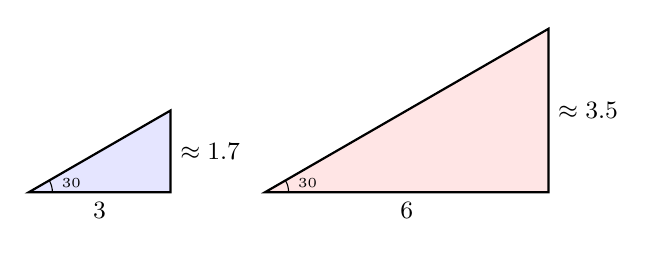
\begin{tikzpicture}[scale=0.6]
  % Small triangle
  \draw[thick,fill=blue!10] (0,0) -- (3,0) -- (3,1.73) -- cycle;
  \node[below] at (1.5,0) {\small $3$};
  \node[right] at (3,0.86) {\small $\approx 1.7$};
  \draw (0.5,0) arc[start angle=0,end angle=30,radius=0.5];
  \node at (0.9,0.2) {\tiny $30°$};
  % Large triangle
  \draw[thick,fill=red!10] (5,0) -- (11,0) -- (11,3.46) -- cycle;
  \node[below] at (8,0) {\small $6$};
  \node[right] at (11,1.73) {\small $\approx 3.5$};
  \draw (5.5,0) arc[start angle=0,end angle=30,radius=0.5];
  \node at (5.9,0.2) {\tiny $30°$};
\end{tikzpicture}
\end{center}
\end{questionText}
\choiceA{SSS produces multiple triangles}
\choiceB{AAA produces a unique triangle}
\choiceC{AAA produces multiple triangles of different sizes}
\choiceD{These two triangles are congruent}
\correctAnswer{C}
\explanation{Both triangles have the same angles but different side lengths. AAA determines shape but not size, so many triangles are possible.}
\end{practiceQuestion}

\begin{practiceQuestion}{6-5-q15}{mc}
\begin{questionText}
A pyramid with a square base is sliced with a horizontal cut near the top. What shape is the cross-section?
\end{questionText}
\choiceA{A very small square}
\choiceB{A triangle}
\choiceC{A point}
\choiceD{A circle}
\correctAnswer{A}
\explanation{A horizontal cut of a square pyramid parallel to the base gives a square. Near the top, the square is very small. At the very apex it would be a point, but a cut ``near the top'' gives a small square.}
\end{practiceQuestion}

\begin{practiceQuestion}{6-8-q04}{mc}
\begin{questionText}
Triangle $PQR \sim$ Triangle $STU$. $PQ = 8$, $ST = 20$, $QR = 6$. Find $TU$.
\end{questionText}
\choiceA{$10$}
\choiceB{$12$}
\choiceC{$15$}
\choiceD{$18$}
\correctAnswer{C}
\explanation{Scale factor: $\frac{20}{8} = 2.5$. $TU = 6 \times 2.5 = 15$.}
\end{practiceQuestion}

\begin{practiceQuestion}{7-4-q17}{mc}
\begin{questionText}
A swimming pool is shaped like a rectangle $25$ m by $10$ m with a semicircle of diameter $10$ m at one end. What is the total area? Use $\pi \approx 3.14$.
\end{questionText}
\choiceA{$250$ m$^2$}
\choiceB{$289.25$ m$^2$}
\choiceC{$328.5$ m$^2$}
\choiceD{$367.75$ m$^2$}
\correctAnswer{B}
\explanation{Rectangle: $25 \times 10 = 250$ m$^2$. Semicircle: $\frac{1}{2} \times 3.14 \times 5^2 = \frac{1}{2} \times 78.5 = 39.25$ m$^2$. Total: $250 + 39.25 = 289.25$ m$^2$.}
\end{practiceQuestion}

\begin{practiceQuestion}{7-5-q26}{gmc}
\begin{questionText}
The net of a rectangular prism is shown below. What is the total surface area?

\begin{center}
\begin{tikzpicture}[scale=0.4]
  % Base cross-shaped net
  \draw[thick,funBlue,fill=funBlue!10] (0,0) rectangle (6,4);
  \node at (3,2) {$6 \times 4$};
  \draw[thick,funBlue,fill=funBlue!10] (6,0) rectangle (9,4);
  \node at (7.5,2) {$3 \times 4$};
  \draw[thick,funBlue,fill=funBlue!10] (9,0) rectangle (15,4);
  \node at (12,2) {$6 \times 4$};
  \draw[thick,funBlue,fill=funBlue!10] (15,0) rectangle (18,4);
  \node at (16.5,2) {$3 \times 4$};
  \draw[thick,funBlue,fill=funBlue!10] (0,4) rectangle (6,7);
  \node at (3,5.5) {$6 \times 3$};
  \draw[thick,funBlue,fill=funBlue!10] (0,-3) rectangle (6,0);
  \node at (3,-1.5) {$6 \times 3$};
\end{tikzpicture}
\end{center}
\end{questionText}
\choiceA{$72$ square units}
\choiceB{$84$ square units}
\choiceC{$108$ square units}
\choiceD{$144$ square units}
\correctAnswer{C}
\explanation{Two $6 \times 4$ faces: $48$. Two $3 \times 4$ faces: $24$. Two $6 \times 3$ faces: $36$. Total: $48 + 24 + 36 = 108$ square units.}
\end{practiceQuestion}

\begin{practiceQuestion}{7-6-q20}{sa}
\begin{questionText}
A cube has a side length of $6$ inches. What is its volume?
\end{questionText}
\correctAnswer{$216$ in$^3$}
\explanation{$V = 6^3 = 216$ in$^3$.}
\end{practiceQuestion}

\begin{practiceQuestion}{8-1-q16}{mc}
\begin{questionText}
Why is a convenience sample (e.g., surveying your friends) usually not a good way to learn about a population?
\end{questionText}
\choiceA{It is too expensive}
\choiceB{It takes too long}
\choiceC{It is likely biased and not representative}
\choiceD{It includes too many people}
\correctAnswer{C}
\explanation{Convenience samples are easy but likely biased because they don't give everyone an equal chance.}
\end{practiceQuestion}

\begin{practiceQuestion}{8-2-q30}{gsa}
\begin{questionText}
The table shows the results of two random samples of $50$ people about their favorite season.

\begin{center}
\begin{tabular}{|l|c|c|}
\hline
\textbf{Season} & \textbf{Sample 1} & \textbf{Sample 2} \\
\hline
Spring & $12$ & $14$ \\
\hline
Summer & $18$ & $16$ \\
\hline
Fall & $10$ & $12$ \\
\hline
Winter & $10$ & $8$ \\
\hline
\end{tabular}
\end{center}

Using both samples, estimate the percent of the population that prefers summer. If the town has $8{,}000$ people, predict how many prefer summer.
\end{questionText}
\correctAnswer{$34\%$; $2{,}720$ people}
\explanation{Summer total: $18 + 16 = 34$ out of $100 = 34\%$. Then $34\%$ of $8{,}000 = 2{,}720$.}
\end{practiceQuestion}

\begin{practiceQuestion}{8-4-q01}{mc}
\begin{questionText}
Data set A: $10, 12, 14, 16, 18$. What is the mean?
\end{questionText}
\choiceA{$12$}
\choiceB{$14$}
\choiceC{$16$}
\choiceD{$70$}
\correctAnswer{B}
\explanation{$\frac{10+12+14+16+18}{5} = \frac{70}{5} = 14$.}
\end{practiceQuestion}

\begin{practiceQuestion}{8-5-q14}{mc}
\begin{questionText}
A back-to-back stem-and-leaf plot is used to:
\end{questionText}
\choiceA{Show one data set with two stems}
\choiceB{Compare two data sets using the same stems}
\choiceC{Display data that has been doubled}
\choiceD{Show data in a circle}
\correctAnswer{B}
\explanation{A back-to-back plot has leaves for one group on the left and for another group on the right, sharing the same stems.}
\end{practiceQuestion}

\begin{practiceQuestion}{8-6-q03}{mc}
\begin{questionText}
A sector of a circle graph represents $25\%$ of the data. What is its angle?
\end{questionText}
\choiceA{$25°$}
\choiceB{$45°$}
\choiceC{$90°$}
\choiceD{$180°$}
\correctAnswer{C}
\explanation{$25\% \times 360° = 0.25 \times 360° = 90°$.}
\end{practiceQuestion}

\begin{practiceQuestion}{9-4-q21}{sa}
\begin{questionText}
A bag has $6$ red, $4$ blue, and $10$ white marbles. Write the probability model by listing $P(\text{red})$, $P(\text{blue})$, and $P(\text{white})$ as fractions in simplest form.
\end{questionText}
\correctAnswer{$P(\text{red}) = \frac{3}{10}$, $P(\text{blue}) = \frac{1}{5}$, $P(\text{white}) = \frac{1}{2}$}
\explanation{Total: $20$. $P(\text{red}) = \frac{6}{20} = \frac{3}{10}$, $P(\text{blue}) = \frac{4}{20} = \frac{1}{5}$, $P(\text{white}) = \frac{10}{20} = \frac{1}{2}$.}
\end{practiceQuestion}

\begin{practiceQuestion}{9-6-q26}{gmc}
\begin{questionText}
The table shows all possible sums when two dice are rolled. What is the probability of rolling a sum of $8$?

\begin{center}
\begin{tabular}{|c|c|c|c|c|c|c|}
\hline
$+$ & \textbf{1} & \textbf{2} & \textbf{3} & \textbf{4} & \textbf{5} & \textbf{6} \\
\hline
\textbf{1} & $2$ & $3$ & $4$ & $5$ & $6$ & $7$ \\
\hline
\textbf{2} & $3$ & $4$ & $5$ & $6$ & $7$ & \cellcolor{funBlue!20}$8$ \\
\hline
\textbf{3} & $4$ & $5$ & $6$ & $7$ & \cellcolor{funBlue!20}$8$ & $9$ \\
\hline
\textbf{4} & $5$ & $6$ & $7$ & \cellcolor{funBlue!20}$8$ & $9$ & $10$ \\
\hline
\textbf{5} & $6$ & $7$ & \cellcolor{funBlue!20}$8$ & $9$ & $10$ & $11$ \\
\hline
\textbf{6} & $7$ & \cellcolor{funBlue!20}$8$ & $9$ & $10$ & $11$ & $12$ \\
\hline
\end{tabular}
\end{center}
\end{questionText}
\choiceA{$\frac{4}{36}$}
\choiceB{$\frac{5}{36}$}
\choiceC{$\frac{6}{36}$}
\choiceD{$\frac{8}{36}$}
\correctAnswer{B}
\explanation{Outcomes with sum $8$: $(2,6), (3,5), (4,4), (5,3), (6,2)$ — that is $5$. $P = \frac{5}{36}$.}
\end{practiceQuestion}

\begin{practiceQuestion}{9-7-q18}{mc}
\begin{questionText}
In a simulation of $100$ free throws, a basketball player makes $78$. If the player's actual success rate is $75\%$, is the simulation result reasonable?
\end{questionText}
\choiceA{No, any difference means the simulation is wrong}
\choiceB{Yes, $78\%$ is close to $75\%$, which is expected variation}
\choiceC{No, because $78$ is not equal to $75$}
\choiceD{Yes, but only if exactly $75$ are made}
\correctAnswer{B}
\explanation{$\frac{78}{100} = 0.78$ vs. theoretical $0.75$. A small difference in $100$ trials is normal and expected.}
\end{practiceQuestion}
